\chapter{Finaal ontwerp}
\label{final}
\section{Het finaal ontwerp}
Het finale ontwerp is een geheugen dat uit 32BL, 32WL en 512GB bestaat. Van de 32 BL worden er 16 gebruikt voor het genereren van het referentiespanning. En van deze 16 zijn er 6 in HRS en 10 en LRS. Dit om de referentiespanningsverdeling beter te centreren tussen de BL-spanningen voor cellen in RHS en LRS. De afmetingen van alle transistoren staan in tabel \ref{tab:transsize}. \\
Op dit geheugen wordt een speed-vdd-test uitgevoerd. Dit is een test waarbij de voedingspanning wordt verlaagt en er vervolgens gekeken wordt aan welke snelheid de leescyclus nog kan uitgevoerd worden. In deze test worden de tijdstippen wanneer de SA aangeschakeld en waneer de uitgang nagekeken werd, onafhankelijk van de voedingspanning bepaalt. Dit geeft een iets optimistisere resultaten dan dat dit door een digitaal circuit zou worden aangestuurd. Figuur \ref{fig:speedvdd} toont de resultaten van deze test. Op elk punt in de figuur werden 100 montecarlo simulatie uitgevoerd. Zoals men duidelijk kan zien  daalt de leessnelheid bij het verlagen van de voedingspanning. Dit komt door een combinatie van 2 zaken. Ten eerste gaat de logica trager worden, dit heeft als gevolg dat de bitlijnen later worden aangestuurd en dat er een verschil ontstaat tussen de aansturing van de bitlijn en woordlijn. Dit verschil uit zich in het snel stijgen van de bitlijn spanning zoals in het vorig hoofdstuk word geillustreerd in figuur \ref{fig:critisch_timing1}. Door deze snelle stijging van de bitlijn moet met langer wachten om het bitlijn voltage van een lage cell uit te lezen. Het tweede fenomeen dat de leessnelheid doet vertragen is de sense amplifier. Bij een voedingspanning van 1V kan de senseamplifier binnen de 0.25ns schakelen. Bij lagere voedingspanningen kan dit afhankelijk van de mismatch to 2ns duren vooralleer de senseamplifier volledig geschakelt is.

\begin{table}
\begin{center}
\begin{tabularx}{\textwidth}{XXX}
\hline
Transistor & L (nm) & W (nm)\\
\hline
ChargeBL & 195 & 300 \\
DischargeBL & 45 & 100 \\
DischargeSL & 45 & 500 \\
Sa enableP & 45 & 900 \\
Sa enableN & 45 & 500 \\
Sa P & 45 & 1700 \\
Sa N & 45 & 1500 \\
Mux LB & 45 & 200 \\
Mux GB & 45 & 100 \\
\hline
\end{tabularx}
\end{center}
\caption{Grotes van de transistoren in het finaal ontwerp}
\label{tab:transsize}
\end{table}
	
\begin{figure}[!ht]
  \centering
  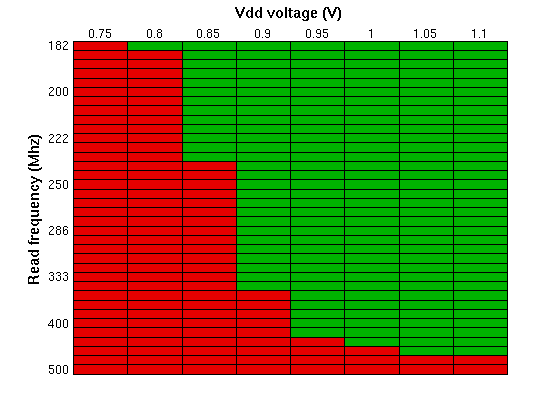
\includegraphics[scale=0.8]{../fig/hfdst-final-vddspeed.png}
  \caption{Resultaten speed-vdd test}
  \label{fig:speedvdd}
\end{figure}

Verder kan men ook zien dat de schakeling een voedingspanning hoger of gelijk aan 0.8V nodig heeft om correct te kunnen werken. De verklaring hiervoor kan gezien worden in figuur \ref{fig:vblvdd}. Deze figuur stelt de distributie voor van de bitlijn spanningen van een cell in RHS, de referentie cellen en een cell in LRS in functie van verschillende voedings spanningen. Er kan duidelijk gezien worden dat bij het verlagen van de voedings spanningen deze distributies dichter bij elkaar komen te liggen en dat een voedingspanning van 0.8V wel degelijk een limiet is. Aangezien de extremas van de distributies bij een voedingspanning van 0.8V zo dicht bij elkaar zitten, word er verder verwacht dat bij deze spanning de schakeling ook ocasioneel zal falen door dat de senseamplifier ontworpen is voor een $\Delta V$ van 35mV. Dit is echter niet opgedoken in de 100 montecarlo simulaties.
Als men naar de bitlijn voltage distributies kijkt voor een voedingspanning van 1V zal men opmerken dat deze niet de zelfde zijn als dezelfde distributie die getoont werden in het hoofdstuk van de last impedatie (figuur \ref{fig:distswitch}). Dit komt door dat men in de speed-vdd test niet wacht to de bitlijn volledig is opgeladen, wat een tijds winst oplevert. Ook werd er in het hoofdstuk van de last impedatie voor gestelt dat er een energie winst zou bereikt kunnen worden door een andere last te kiezen (sectie \ref{anderelast}). Hoewel dit mogelijk is, heeft dit wel als nadeel dat de schakeling minder tolerant zal zijn voor voedingspanning verschillen. Ten slotte moet ook vermeld worden dat de speed-vdd test uitgevoerd werd op een (spice) temperatuur van $30^{\circ}\mathrm{C}$. Moest deze schakeling worden geimplementeert in een processor is de kans groot dat dit onderhevig zal zijn aan temperaturen tussen de $30^{\circ}\mathrm{C}$ en $60^{\circ}\mathrm{C}$ wat ook een tragere leest snelheiden zal opleveren. Hoe traag, werd echter niet onderzocht.

\begin{figure}[!ht]
  \centering
  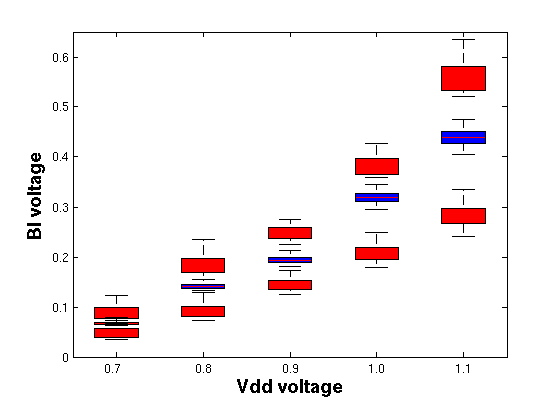
\includegraphics[scale=0.8]{../fig/hfdst-final-vddbl.png}
  \caption{Bl spanningen ifv Vdd}
  \label{fig:vblvdd}
\end{figure}

Het totale energie verbruik van een leescyclus bij een voeding spanning van 1V is gemiddelt 0.51pJ. Hier bij gaat 25\% van de energie naar de logic, 2\% naar de senseamplifier, 65\% naar de bitlijnen en 8\% naar de buffers. Hier bij werden de buffers in de decoders bij de logic gerekent.

\section{Vergelijking met de literatuur}
Het vergelijken van 2 chips is geen evidentie. Ten eerste verschillen vaak de vooropgestelde chip specificaties, ten tweede verschillen vaak de technologieën en tenslotte geven veel papers niet alle resultaten weer om goed te kunnen vergelijken. Chipspecificaties hangen af van de noden van de applicatie van de chip. Voor automotive applicaties bijvoorbeeld is er vooral nood aan geheugens die bij hoge temperaturen een hoge betrouwbaarheid hebben. Medische toepassingen daarentegen hebben  nood aan low-power chips. Onder verschillende technologieën kan er een onderscheid gemaakt worden tussen de technologie van de logica en van het geheugen. Zo wordt er vaak voor verschillende toepassingen een andere soort NOR-flash geheugencel gebruikt: charge-trapping-cellen worden gebruikt voor betere betrouwbaarheid, split-gates-cellen voor hoge performantie \cite{5783209}. De schakeling ontworpen in dit werk kan bij de snellere geheugens worden gecategoriseerd vergeleken met NOR-geheugens in de industrie \cite{6649105}\cite{4433985}\cite{4027813}. Hierbij werd er gekeken naar de random-access-leessnelheid. Vaak kan een groot verschil in leessnelheid ook voor een deel verklaart worden door een andere capaciteit op de bitlijn. Vermids het energieverbruik berekend kan worden doormiddel van $CV_{vdd}^{2}$ kan men vermoeden dat de schakeling in dit werk ook bij de meer energiezuinige schakelingen hoort. De meeste schakelingen gevonden in de literatuur hebben namelijk een hogere voedingsspanning. De werking van het memristor geheugen op verschillende temperaturen werd in dit werk niet onderzocht. Naast verschillen in de werking van de logica, zal ook de memristor onderhevig zijn aan temperatuurs veranderingen. Volgens \cite{5948374} zal bij een $HfO_{2}$ geheugen cell de $ROFF/RON$ verhouding dalen bij stijgende temperatuur. Ondanks deze daling in performatie, ziet men in de industrie toch RRam-chips opduiken die werken bij hoge temperaturen\footnote{http://www.crossbar-inc.com/markets/automotive.html}. In conclusie kan gezegt worden dat met de aspecten waarin rekening gehouden werd in dit werk, de schakeling een goede prestatie levert tov schakelingen in de literatuur.

\section{Besluit}
Een finale schakeling werd ontworpen en geëvalueerd. Hierbij werd er voornamelijk gekeken naar de prestatie onder verschillende voedingsspanningen. Er werd een absolute limiet van 0.8V gevonden voor de voedings spanning en verklaart. Verder werd er gekeken naar Nor-flash schakelingen in de literatuur en werd er besloten dat de schakeling in dit werk een goede concurent is op het vlak van snelheid en energieverbruik. Andere aspecten konden niet met zekerheid vergeleken worden aangezien deze niet onderzocht werden in dit werk.